\documentclass[../main.tex]{subfiles}
Durante este capítulo, se presentará el caso de estudio en su conjunto. Empezando por la aplicación específica y la motivación de la misma, además del modelo utilizado para dicha aplicación. Siguiendo con la solución obtenida y la discusión de esta. Por último, se propondrá una aproximación a un sistema concreto, haciendo uso de la soluciones obtenidas previamente, como resolución al problema presentado. 

\section{Aplicación} \label{section:aplicacion}
En este estudio se han seleccionado los micro-vehículos aéreos, de ahora en adelante MAVs (\emph{Micro Aerial Vehicles}), como aplicación concreta sobre la que realizar la taxonomía. Un MAV es aquel vehículo aéreo autónomo con un peso inferior a 50g \cite{mcguire.2017}. También son conocidos como drones de bolsillo o \emph{pocket drones}. \\

\begin{figure}[h]
    \begin{subfigure}{0.5\textwidth}
        \includegraphics[height=6cm, width=0.9\linewidth]{photos/jjrc-h36.PNG}
        \caption{JJRC H36 \cite{h36}.}
        \label{fig:h36}
    \end{subfigure}
    \begin{subfigure}{0.5\textwidth}
        \includegraphics[height=6cm, width=0.9\linewidth]{photos/e010_mano.jpg}
        \caption{Eachine E010 \cite{e010}.}
        \label{fig:e010}
    \end{subfigure}
     
    \caption{MAVs propuestos para la aplicación.}
    \label{fig:mavs}
\end{figure}

Esta decisión viene motivada debido a un posible proyecto futuro en la Universidad Rey Juan Carlos (URJC). El proyecto en cuestión trata sobre el desarrollo de un circuito de MAVs recreativo con un solo grado de libertad, la velocidad. El circuito trataría de simular al ya existente circuito en tierra (\emph{scalextric} \cite{scalextric}). Aunque tenga sus similitudes, el desafío es mucho mayor, pues no existen guías que puedan seguir los vehículos y por la necesidad de un sistema de posicionamiento ligero, preciso y de bajo coste. Ligero pues un MAV no puede tener una carga elevada sin que limite su autonomía o su maniobrabilidad. Barato pues con un uso recreativo, se busca que sea accesible también en coste. Y preciso pues al ser vehículos de pequeño tamaño, el error admisible debe ser también reducido. \\
En concreto, un ejemplo de un MAV utilizado para esta aplicación sería el Eachine E010 (Fig. \ref{fig:e010}) o el JJRC H36 (Fig. \ref{fig:h36}). \\

Es el momento de recuperar la Tabla \ref{table:explanation} y justificar el rango de valores asociado a cada propiedad. Los drones propuestos tienen unas características concretas que condicionan su vuelo. Poseen una masa de 19g (E010) y de 22g (H36) lo que limita la carga de pago. Además, su pequeño tamaño 9,5x9,5x5cm (E010) y 8,5x8,5x3cm (H36) no permite errores en el posicionamiento elevados. En la siguiente Tabla \ref{table:mavs} se resumen las características comentadas: \\

\begin{table}[h]
    \centering
    \begin{threeparttable}
        \begin{tabular}{l c c}
            \toprule
             & \thead{Eachine E010} & \thead{JJRC H36} \\
            
            \midrule
            Masa (g) & 19 & 22 \\
            Tamaño (cm) & 9,5x9,5x5 & 8,5x8,5x3 \\
            
            \bottomrule
            \addlinespace[1ex]
        \end{tabular}
        
    \end{threeparttable}
    
    \caption{Propiedades de los MAVs propuestos para la aplicación.}
    \label{table:mavs}
\end{table}

\subsection*{Modelo utilizado} \label{subsection:mod_app}
A la hora de definir el modelo utilizado, se han fijado los correspondientes coeficientes con los siguientes valores:

\begin{align}
    \alpha   & = 3 & \gamma  & = 1 & \mu & = 1 & \omega & = 0 \nonumber \\
    \beta    & = 1 & \delta  & = 1 & \nu  & = 3 & & \label{eq:coef}
\end{align} 

Partiendo de la Ecuación \ref{eq:modelo} y aplicando los coeficientes anteriores \ref{eq:coef}, se obtiene el siguiente modelo final:

\begin{equation}
    3 CP + IM + UF + RAN + 3 POS + ACT
    \label{eq:modelo_final}
\end{equation}

El añadir pesos a los diferentes requisitos permite valorar con distinta relevancia las cualidades llevadas al análisis. De esta forma, es fácil observar que las propiedades más relevantes para este estudio son la carga de pago y la exactitud en el posicionamiento con un coeficiente de valor \emph{tres}. En segundo lugar, estaría el coste con un peso de valor \emph{dos}, pues este está dividido en el coste de infraestructura y de usuario. Por último, se encuentran el rango y la actitud con peso igual a la \emph{unidad}. \\
Los pesos aplicados a cada requisito concuerda con lo introducido en la sección anterior (\ref{section:aplicacion}), donde se mencionó la importancia de la carga de pago y de la precisión debido al tamaño y peso limitado de los drones seleccionados. El coeficiente asociado al coste recibe dicha relevancia debido a que su aplicación se ubica en un mercado de uso recreativo donde el objetivo es alcanzar el mayor público con coste reducido. Además, el precio de estos drones tampoco es elevado y se busca una solución acorde al precio de los mismos.

\section{Solución} \label{section:solucion}
Para concluir esta sección se presenta una nueva Tabla \ref{table:comparat} como solución a esta aplicación concreta. Teniendo como origen la Tabla \ref{table:taxonomy}, sustituyendo sobre esta las valoraciones por sus valores numéricos asociados (Tabla \ref{table:baremo}) y aplicando el modelo establecido en la Ecuación \ref{eq:modelo_final}, se obtiene la nueva Tabla \ref{table:comparat}. \\

\afterpage{
\begin{landscape}
    
    \begin{ThreePartTable}
    \renewcommand\TPTminimum{\textwidth}
    %% Arrange for "longtable" to take up full width of text block
    \setlength\LTleft{0pt}
    \setlength\LTright{0pt}
    \setlength\tabcolsep{0pt}
    
    \begin{longtable}{ l @{\extracolsep{\fill}} *{8}{c} }
    
    \caption{Soluciones obtenidas para las tecnologías IPS.}
    \label{table:comparat}\\
    \toprule
                               & \thead{Carga}   & \multicolumn{2}{c}{\thead{Coste}} &               & \thead{Posicionamiento} & \thead{Actitud} & \thead{Obstáculos} & \multirow{2}{*}{\thead{TOTAL}} \\
            \thead{Tecnología} & \thead{de pago} & \thead{IM}           & \thead{UF} & \thead{Rango} & \thead{(Exactitud)}     & \thead{(Si/no)} & \thead{(Si/No)}    &                                \\
    \midrule
    \endfirsthead
    
    \multicolumn{6}{c}{{\textit{\tablename\ \thetable{} -- continuación de la hoja anterior} }}\\
    \toprule
                               & \thead{Carga}   & \multicolumn{2}{c}{\thead{Coste}} &               & \thead{Posicionamiento} & \thead{Actitud} & \thead{Obstáculos} & \multirow{2}{*}{\thead{TOTAL}} \\
            \thead{Tecnología} & \thead{de pago} & \thead{IM}           & \thead{UF} & \thead{Rango} & \thead{(Exactitud)}     & \thead{(Si/no)} & \thead{(Si/No)}    &                                \\
    \midrule
    \endhead

    \midrule[\heavyrulewidth]
    \multicolumn{8}{r}{\textit{---continua en la siguiente hoja}}\\
    \endfoot  

    \midrule[\heavyrulewidth]
    \endlastfoot
        
        Infrarrojos         & 2 & 3 & 1 & 0 & 1 & 0 & 0 & \textbf{4,33} \\ \\
        
        Luz visible         & 3 & 0 & 2 & 0 & 1 & 0 & 0 & \textbf{4,42} \\ \\
        
        \emph{Optical flow} & 1 & 3 & 0 & 1 & 2 & 1 & 0 & \textbf{6,75} \\ \\
        
        \emph{Optical motion}  & \multirow{2}{*}{4} & \multirow{2}{*}{1} & \multirow{2}{*}{3} & \multirow{2}{*}{0} & \multirow{2}{*}{2} & \multirow{2}{*}{0} & \multirow{2}{*}{0} & \multirow{2}{*}{\textbf{7,33}} \\
        \emph{tracking}        &                    &                    &                    &                    &                    &                    &                    & \\ \\
            
        \emph{Optical marked}  & \multirow{2}{*}{4} & \multirow{2}{*}{0} & \multirow{2}{*}{2} & \multirow{2}{*}{0} & \multirow{2}{*}{2} & \multirow{2}{*}{1} & \multirow{2}{*}{1} & \multirow{2}{*}{\textbf{7,67}} \\
        \emph{motion tracking} &                    &                    &                    &                    &                    &                    &                    & \\ \\
            
        \emph{Marked-based}    & \multirow{2}{*}{2} & \multirow{2}{*}{2} & \multirow{2}{*}{0} & \multirow{2}{*}{1} & \multirow{2}{*}{2} & \multirow{2}{*}{1} & \multirow{2}{*}{0} & \multirow{2}{*}{\textbf{7,17}} \\
        (Activo)               &                    &                    &                    &                    &                    &                    &                    & \\ \\
        
        \emph{Marked-based}    & \multirow{2}{*}{4} & \multirow{2}{*}{0} & \multirow{2}{*}{2} & \multirow{2}{*}{0} & \multirow{2}{*}{2} & \multirow{2}{*}{1} & \multirow{2}{*}{0} & \multirow{2}{*}{\textbf{7,67}} \\
        (Pasivo)               &                    &                    &                    &                    &                    &                    &                    & \\ \\
        
        \emph{Vision-based} & 1 & 3 & 1 & 1 & 2 & 1 & 1 & \textbf{7,08} \\ \\

        LiDAR               & 0 & 3 & 0 & 1 & 2 & 0 & 1 & \textbf{5,00} \\ \\

        Ultrasonidos        & 2 & 2 & 1 & 1 & 2 & 0 & 0 & \textbf{6,50} \\ \\
        
        Audible             & 2 & 2 & 1 & 0 & 1 & 0 & 0 & \textbf{4,00} \\

        Magnética           & 4 & 0 & 3 & 0 & 0 & 0 & 0 & \textbf{4,00} \\ \\

        WLAN                & 2 & 2 & 0 & 1 & 0 & 0 & 0 & \textbf{3,17} \\ \\

        Bluetooth           & 2 & 1 & 1 & 1 & 0 & 0 & 0 & \textbf{3,17} \\ \\

        RFID activo         & 1 & 2 & 0 & 1 & 0 & 0 & 0 & \textbf{2,42} \\ \\

        RFID pasivo         & 3 & 0 & 2 & 0 & 0 & 0 & 0 & \textbf{2,92} \\ \\

        UWB                 & 3 & 1 & 1 & 1 & 1 & 0 & 0 & \textbf{5,42} \\ \\

        IMU                 & 2 & 3 & 1 & 1 & 2 & 1 & 0 & \textbf{7,83} \\ 
    \end{longtable}   
    \end{ThreePartTable}
\end{landscape}
}

Para una mejor visualización de los datos, se añade una nueva tabla (Tab. \ref{table:resumen}) con las mejores soluciones ordenadas por la nota obtenida. Es importante mencionar que la puntuación máxima es diez, pues se tuvo en consideración a la hora de construir el modelo para evitar posibles confusiones.

\begin{table}[H]
    \centering
    \begin{threeparttable}
        \begin{tabular}{l c}
            \toprule
            \thead{Tecnología} & \thead{Total} \\
            
            \midrule
            IMU                           & 7,83 \\
            \emph{Marked motion tracking} & 7,67 \\
            \emph{Marked-based} (Pasivo)  & 7,67 \\
            \emph{Motion tracking}        & 7,33 \\
            \emph{Marked-based} (Activo)  & 7,17 \\
            \emph{Vision-based}           & 7,08 \\
            \emph{Optical flow}           & 6,75 \\
            Ultrasonidos                  & 6,50 \\
            UWB                           & 5,42 \\
            
            \bottomrule
            \addlinespace[1ex]
        \end{tabular}
        
    \end{threeparttable}
    
    \caption{Resumen de las soluciones obtenidas para las tecnologías IPS.}
    \label{table:resumen}
\end{table}

La tecnología con mayor puntuación es la IMU, núcleo de muchos sistemas de posicionamiento \cite{li.2018novel}, pero que raramente se utiliza en solitario, pues suele integrarse en sistemas híbridos \cite{benini.2013, zhou.2018vslam, gageik.2013}. Las siguientes tecnologías son todas dispositivos ópticos, finalizando con dos tecnologías de RF, ultrasonidos y UWB. El resultado obtenido concuerda con las tendencias actuales en los IPS, pues la mayoría de productos \cite{li.2018novel}, tanto en fase de desarrollo como en fase comercial, utilizan tecnologías ópticas (híbridas) para determinar el posicionamiento. \\
Sobre las soluciones obtenidas, es necesario realizar un filtrado previo, pues alguna solución es inviable. Por un lado, debido a un coste asociado inasequible, se excluye \emph{Marked motion tracking}. Por otro lado, debido a una carga de pago excesiva, se excluyen \emph{Optical flow}, la navegación basada en marcadores (activo) y la navegación basada en visión, donde el drone no podría actuar debido al peso de la carga. \\
Este filtrado no se ha realizado previo al análisis debido a la intención del estudio de ser lo más general posible, y es ahora en última instancia cuando descartamos estas soluciones obtenidas para nuestra aplicación aunque hayan obtenido puntuaciones destacadas. \\
Entre las tecnologías restantes, se propone una solución concreta y se estudian sus alternativas en la siguiente Sección \ref{section:sistema}.

\clearpage % OJO
\subsection{Discusión}
Previo a desarrollar el sistema-solución, sobre los resultados obtenidos se quiere realizar un análisis que permita entender la validez y el porqué de los mismos. \\

Buscando robustez sobre las soluciones obtenidas, se plantean otros modelos con diferentes coeficientes para contrastar resultados. Los nuevos modelos propuestos sobre los que aplicaremos la misma comparativa son los formulados en las Ecuaciones \ref{eq:modelo_1} y \ref{eq:modelo_2}.

\begin{equation}
    4 CP + 3 IM + 3 UF + 2 RAN + 2 POS + ACT
    \label{eq:modelo_1}
\end{equation}

El primer modelo (Ecuación \ref{eq:modelo_1}) puede parecer extraño por los coeficientes utilizados, pero es el resultante si los valores de las propiedades no estuvieran normalizados. Es un modelo muy sencillo pues es producto de la suma de los valores del baremo asociados a cada propiedad.

\begin{equation}
    CP + IM + UF + RAN + POS + ACT
    \label{eq:modelo_2}
\end{equation}

El segundo modelo (Ecuación \ref{eq:modelo_2}) es también muy simple. Todos los coeficientes son iguales, es decir, todas las propiedades tienen la misma relevancia. \\
El tercer modelo es el utilizado para construir la Tabla \ref{table:comparat} y con el que se han obtenido los resultados aquí discutidos. La ecuación del modelo se puede rescatar de la Ecuación \ref{eq:modelo_final}. \\

La siguiente gráfica (Fig. \ref{fig:grafico}) muestra la puntuación obtenida de cada tecnología en función del modelo utilizado. Los resultados están organizados según su puntuación obtenida para facilitar su comprensión.

\begin{figure}[h]
    \centering
    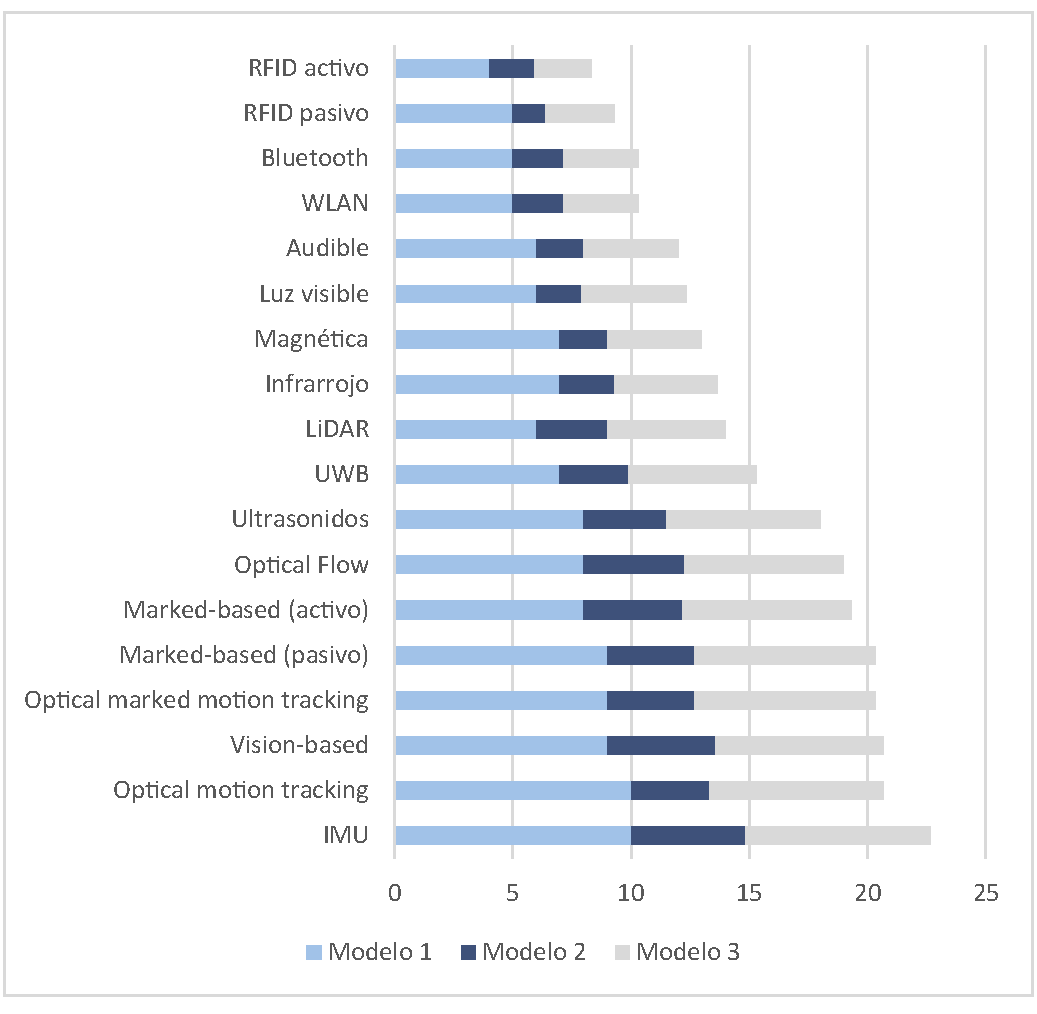
\includegraphics[width=0.92\textwidth]{grafico.pdf}
    \caption{Resultados obtenidos en función del modelo aplicado.}
    \label{fig:grafico}
\end{figure}

Se puede observar como las mejores soluciones coinciden con las presentadas en la Tabla \ref{table:resumen}, lo cual era esperado, pues son un reflejo de las tendencias actuales. En ambos casos, la solución que reina la clasificación es la IMU, seguido por soluciones basadas en dispositivos ópticos que varían en su orden pero con una puntuación muy próxima entre ellos. En los siguientes puestos se encuentran los sistemas de ultrasonidos y UWB, seguidos por el resto de sistemas. \\
Al igual que hicimos anteriormente, a modo de resumen se presenta una tabla (Tab. \ref{table:res_graf} que recoge los mejores resultados con su puntuación obtenida. Esta puntuación es la resultante de la suma de puntuaciones obtenidas en cada uno de los modelos y dividida entre el numero de modelos, para que la puntuación máxima siga siendo diez. Como ya se ha avanzado, los resultados son muy similares a los obtenidos en la anterior tabla resumen (Tab. \ref{table:resumen}).

\begin{table}[H]
    \centering
    \begin{threeparttable}
        \begin{tabular}{l c}
            \toprule
            \thead{Tecnología} & \thead{Total} \\
            
            \midrule
            IMU                           & 7,56 \\
            \emph{Motion tracking}        & 6,89 \\
            \emph{Vision-based}           & 6,89 \\
            \emph{Marked motion tracking} & 6,78 \\
            \emph{Marked-based} (Pasivo)  & 6,78 \\
            \emph{Marked-based} (Activo)  & 6,44 \\
            \emph{Optical flow}           & 6,33 \\
            Ultrasonidos                  & 6,00 \\
            UWB                           & 5,11 \\

            \bottomrule
            \addlinespace[1ex]
        \end{tabular}
        
    \end{threeparttable}
    
    \caption{Resumen de las soluciones obtenidas aplicando los tres modelos.}
    \label{table:res_graf}
\end{table}

Tras esta breve discusión, se da paso a presentar la solución final que trata de dar solución al problema.

\section{Sistema propuesto} \label{section:sistema}
El sistema que se propone es una solución híbrida que utiliza las tecnologías IMU y UWB. Por un lado, los sistemas inerciales aportan una buena robustez con una alta precisión, pero son muy sensibles a errores, los cuales se acumularán e incrementaran progresivamente. Por otro lado, los sistemas basados en UWB poseen una precisión intermedia pero una posición absoluta discontinua que permite corregir la acumulación de errores de la IMU. Es decir, mediante la hibridación de sistemas conseguimos un sistema robusto, de alta precisión y menos sensible a los errores. En la Figura \ref{fig:hibrid} se trata de representar los motivos que han conducido a esta solución. \\
Además, el coste seguiría siendo moderado, con escalabilidad en la cobertura y con detección de la orientación. Sin embargo, la carga de pago aumenta, al estar embarcando dos sistemas. Se estima que el peso final, pese a ser mayor, seguiría estando dentro del rango aceptable descrito.

\begin{figure}[ht]
    \centering
    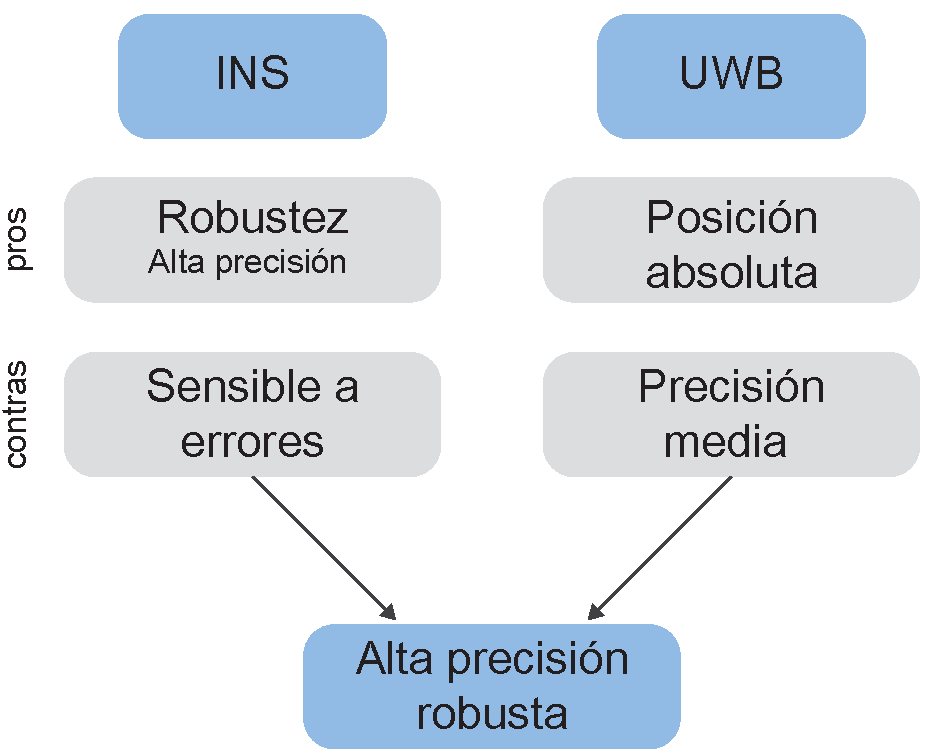
\includegraphics[width=0.6\linewidth]{tradeoffs.pdf}
    \caption{Motivación de la hibridación en la solución.}
    \label{fig:hibrid}
\end{figure}

%\clearpage % OJO, solucion poco elegante

Durante el proceso de búsqueda de la solución, se han valorado otras posibles soluciones, las cuales se presentan a continuación:

\begin{itemize}
    \item Ultrasonidos + IMU
    \item \emph{Motion tracking} + IMU
    \item \emph{Marked-based} (Pasivo) + IMU
    \item \emph{Motion tracking}
\end{itemize}

Si sometemos las soluciones híbridas al modelo para compararlas entre sí podremos observar si la decisión tomada es correcta. Se aporta la Tabla \ref{table:res_hib} con los resultados obtenidos. \\

Como se puede observar la solución elegida obtiene la mejor posición, a continuación se explicarán los principales motivos de la elección. Previamente se quiere aclarar que aunque la solución híbrida haya obtenido una puntuación inferior a un sistema no híbrido, la solución propuesta aporta una robustez inexistente en el resto de alternativas sin sacrificar precisión. \\

\begin{table}[h]
    \centering
    \begin{threeparttable}
        \begin{tabular}{l c}
            \toprule
            \thead{Sistema} & \thead{Total} \\
            
            \midrule
            UWB + IMU                           & 7,17 \\
            Ultrasonidos + IMU                  & 6,75 \\
            \emph{Motion tracking} + IUM        & 6,17 \\
            \emph{Marked-based} (Pasivo) + IMU  & 5,83 \\

            \bottomrule
            \addlinespace[1ex]
        \end{tabular}
        
    \end{threeparttable}
    
    \caption{Resumen de las soluciones obtenidas aplicando los tres modelos.}
    \label{table:res_hib}
\end{table}

Antes de desarrollar el sistema elegido, es necesario explicar el porqué de la decisión y los motivos que han conducido a la misma. \\
En primer lugar, se ha descartado la solución híbrida compuesta por ultrasonidos e IMU debido a que la carga de pago asociada a un equipo de ultrasonidos es ligeramente superior a la de UWB, mientras que la mejoría en precisión no es suficientemente superior para justificar su elección. Las siguientes dos opciones basadas en sistemas híbridos constituidos por dispositivos ópticos (\emph{motion tracking} o \emph{marked-based} pasivo) e IMU, se han descartado debido al coste asociado a los dispositivos ópticos de los sistemas, el cual excede en gran medida al coste de UWB. Por último, la cuarta opción formada \emph{motion tracking} únicamente, pese a aportar una carga de pago y una precisión reseñables, carecen de la robustez que aportan los sistemas inerciales y sufren en situaciones de poca visibilidad debido a la iluminación o a posibles oclusiones parciales o totales. \\
Por estos motivos, se ha decidido apostar por la solución ya presentada, en la cual se profundizará en la siguiente sección (Sec. \ref{subsection:fusion}). Otras soluciones con estos sistemas han sido presentadas por otros autores, entre las que destacan las propuestas por \emph{Paredes et al.} \cite{paredes.2018} y \emph{Wang et al.} \cite{wang.2017ref}. La primera solución propone un sistema compuesto por ultrasonidos y \emph{motion tracking}, mientras que el segundo está compuesto por un escáner láser y UWB.

\subsection*{Fusión de sensores} \label{subsection:fusion}
Como se ha explicado en la sección anterior, la estrategia a seguir será la fusión de dos tecnologías. Por ello, la posición es determinada mediante dos sensores, tal como se muestra en la Figura \ref{fig:fusion}.

\begin{figure}[h]
    \centering
    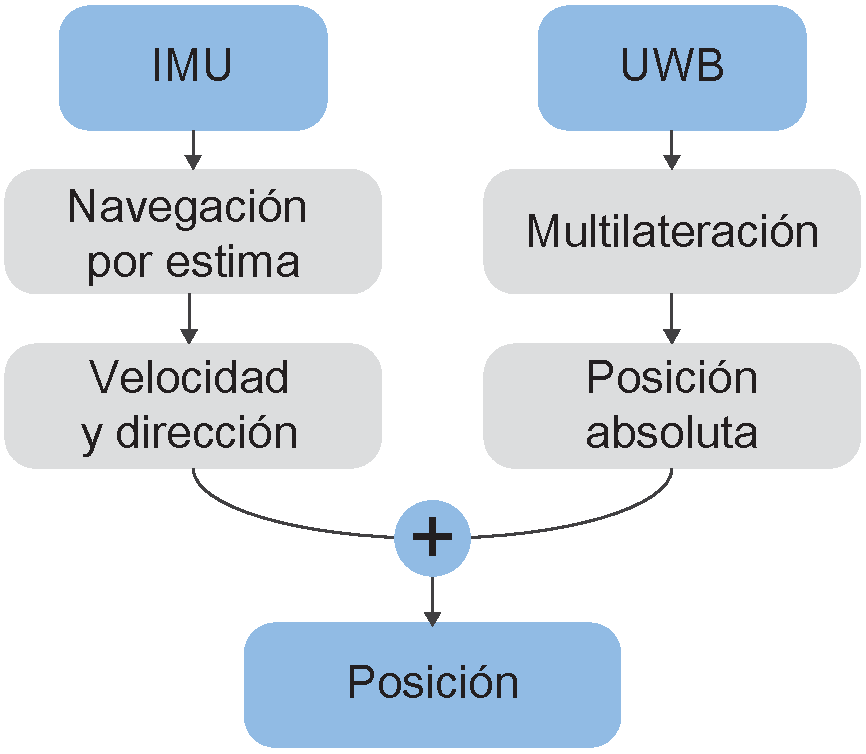
\includegraphics[width=0.6\linewidth]{sensor_fusion.pdf}
    \caption{Integración de sensores.}
    \label{fig:fusion}
\end{figure}

Al integrar las dos tecnologías para la obtención de la posición, también se está fusionando dos algoritmos de posicionamiento diferentes. Por un lado, la IMU utiliza la navegación inercial para obtener la velocidad y dirección en cada instante, con el que podemos integrar la posición en cada momento. Por otro lado, UWB hace uso de la multilateración para calcular la posición absoluta. La resolución de esta posición depende de la frecuencia de transmisión del sistema, que influye de forma directa en el consumo del mismo. El método de fusión de ambas posiciones se explicará más adelante. \\
Con el objetivo de introducir el proceso de integración, en las siguientes secciones se muestran sendos esquemas con una introducción a las arquitecturas hardware y software propuestas. Debido la extensión de este trabajo no se presentan esquemas completos, sino una primera aproximación que debe ser completada para una correcta resolución del problema.

\subsubsection*{Hardware}
El hardware consistiría en un equipo a bordo compuesto por una IMU, un emisor UWB, un pequeño procesador y una antena para la transmisión. En el entorno se situarían varios puntos UWB con antenas receptoras que triangularían la posición del drone \cite{cisek.2017uwb}. Además, el drone establecería una conexión con una estación en tierra (PC), la cual realizaría los cálculos del posicionamiento y recibiría instrucciones de vuelo. En la Figura \ref{fig:hardware} se muestra un esquema que trata de representar el sistema físico propuesto.

\begin{figure}[h]
    \centering
    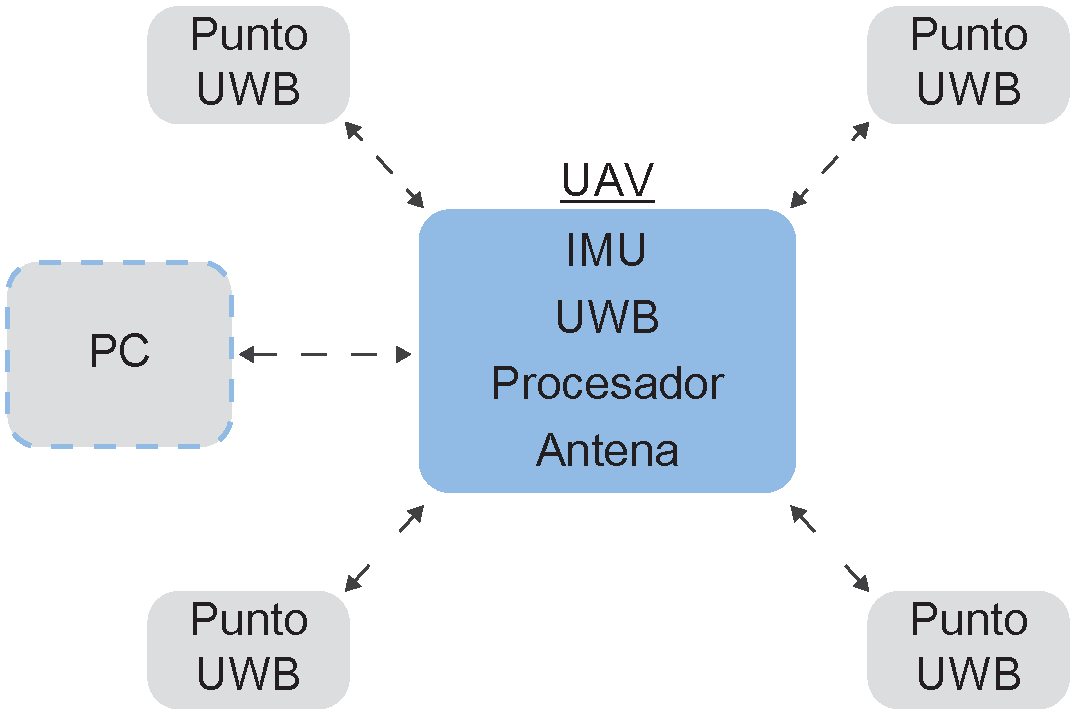
\includegraphics[width=0.6\linewidth]{hardware.pdf}
    \caption{Esquema hardware del sistema propuesto.}
    \label{fig:hardware}
\end{figure}

Es en la estación en tierra donde se ejecutaría el software de integración de datos de ambos sensores. La información de la IMU sería transmitida a través de la antena de abordo del drone, mientras que la triangulación de la posición UWB se realizaría en la misma estación. En la siguiente sección se presenta un esquema para esclarecer el proceso de fusión de datos en sí. \\

\begin{figure}[h]
    \begin{subfigure}{0.5\textwidth}
        \includegraphics[height=6cm, width=0.9\linewidth]{photos/imu.jpg}
        \caption{MiniIMU-9 v5 \cite{imu}.}
        \label{fig:imu}
    \end{subfigure}
    \begin{subfigure}{0.5\textwidth}
        \includegraphics[height=6cm, width=0.9\linewidth]{photos/DWM1000-Module.jpg}
        \caption{DWM1000 Module \cite{dwm1000}.}
        \label{fig:dwm1000}
    \end{subfigure}
     
    \caption{Componentes propuestos para la solución.}
    \label{fig:componentes}
\end{figure}

Con respecto a los componentes necesarios se propone utilizar una \emph{MiniIMU-9 v5} \cite{imu} y un transceptor UWB \emph{DWM1000 Module} \cite{dwm1000}. La IMU propuesta posee un giróscopo de tres ejes, un acelerómetro de tres ejes y un compás magnético de tres ejes integrados en una placa pequeña. Ambos elementos respetan el tamaño, el peso y el precio establecidos en la tabla \ref{table:taxonomy}. En la Figura \ref{fig:componentes} se muestran ambos componentes. \\


\subsubsection*{Software}
La integración de posiciones para obtener una única posición mejorada se realizaría mediante un algoritmo de fusión. Con el objetivo de ilustrar este proceso, se aporta la Figura \ref{fig:software}. \\

\begin{figure}[h]
    \centering
    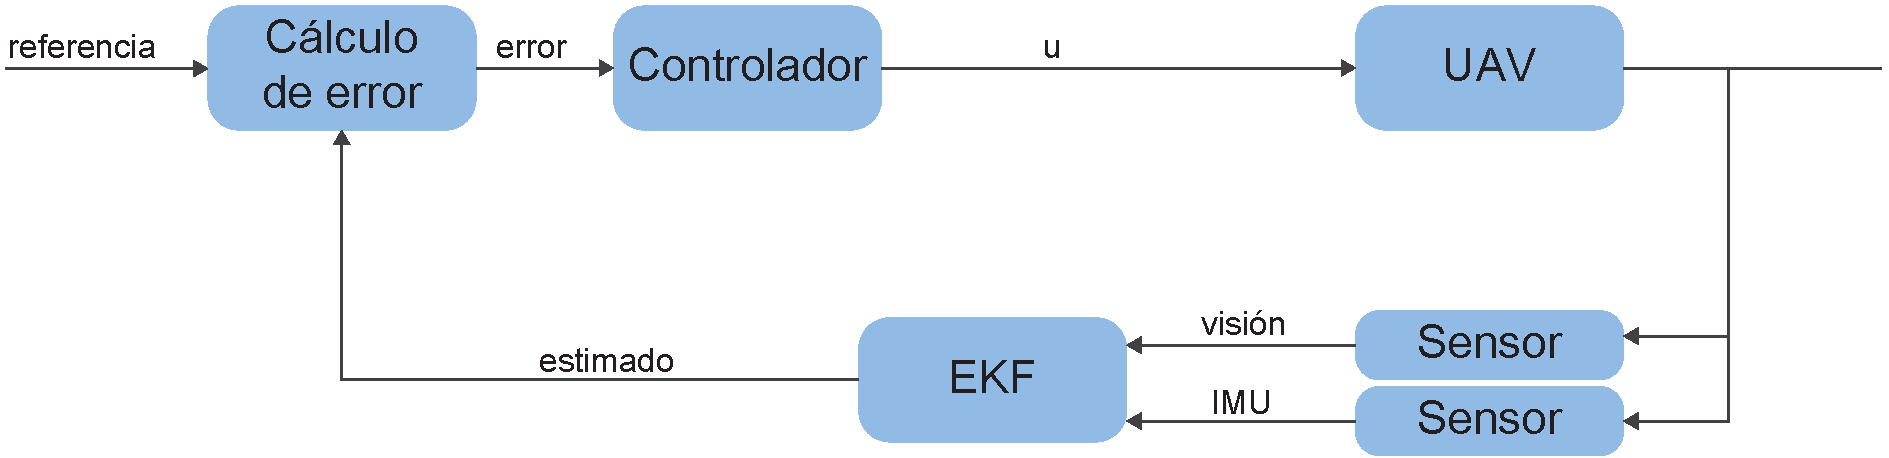
\includegraphics[width=0.9\linewidth]{software.pdf}
    \caption{Esquema software del sistema propuesto.}
    \label{fig:software}
\end{figure}

El proceso estaría compuesto por un bucle retro-alimentado por la información de ambos sensores, IMU e UWB. Para fusión de estos datos se propone un filtro de Kalman extendido (EKF). Se propone utilizar un filtro de Kalman extendido en lugar de un filtro de Kalman básico debido a la no linealidades asociadas al problema. Por otro lado, al estar los modelos de transición bien definidos, no es necesario precisar de un UKF (\emph{Unscented Kalman Filter}). Además, este tipo de filtros (EKF) son ampliamente utilizados en los sistemas de navegación y sistemas GPS \cite{wan.2006ekf}. Gracias al filtro de Kalman se obtendría una posición estimada del drone, que junto a una posición de referencia, es posible estimar el error en el seguimiento de la trayectoria. A través de un controlador, se trataría de eliminar este error transmitiendo al drone las instrucciones necesarias para ello. Existen diversas opciones a la hora de seleccionar el controlador a utilizar, un PID podría ser utilizado como propone \emph{Wang et al.} en su estudio \cite{wang.2017ref} u otros controladores más complejos como MPC entre otros.